% !TEX root = ../../report.tex
\section{Das Terrain}
\begin{Spacing}{\mylinespace}

Nachdem das Grundgerüst der Anwendung stand und wir die Kinect Kamera erfolgreich eingebunden hatten ging es daran uns um die Umsetzung der Terraindarstellung zu kümmern.

\subsection{Die Grundgeometrie}
Als Grundgeometrie für die Darstellung unseres Terrains erzeugen wir ein flaches reguläres Gitter, dass in der X-Z-Ebene aufgespannt ist (s. Abbildung \ref{fig:grid}). Die Größe und die Anzahl der Unterteilungen des Gitters wurde variabel gestaltet, um im späteren Verlauf der Entwicklung, einfacher unterschiedliche Konfiguration zu testen. 

\begin{figure}[h!]
	\centering
	\vspace*{10px}
	\includegraphics[width=0.6\textwidth]{graphics/grid.png}
	\caption{Reguläres Gitter des Terrains.}
	\label{fig:grid}
\end{figure}

\subsection{Die Höhendaten}
Um mit dem zuvor erstellten regulären Gitter ein vollständiges Abbild unserer Sandkastenlandschaft zu repräsentieren, musste nun noch ein Weg gefunden werden die von der Kinect gelieferten Höhendaten in das Model zu integrieren. Abbildung \ref{fig:resize} zeigt die erhaltenen Daten der Kinect.
\\
\begin{figure}[h!]
	\centering
	\includegraphics[width=0.6\textwidth]{graphics/resize.png}
	\caption{Die gelieferten Daten.}
	\label{fig:resize}
\end{figure}  

Um die vorarbeitenden Daten nun auf das reguläre Gitter zu übertragen, kamen zwei unterschiedliche Ansätze in Frage:
\begin{description}
	\item[1. Mit Hilfe der CPU] \hfill \\
	Beim ersten Ansatz werden die Daten direkt auf der CPU verarbeitet und in das reguläre Gitter integriert. Ein großer Nachteil dieses Ansatzes ist allerdings, dass bei jeder Aktualisierung der sogenannte \textit{VertexBuffer}, mit dessen Hilfe die Geometriedaten an die GPU übertragen werden, komplett neu aufgebaut werden muss. Dieser Vorgang ist sehr kostenintensiv und würde die Echtzeitfähigkeit unserer Anwendung stark einschränken.
	\item[2. Mit Hilfe der GPU] \hfill \\
	Beim zweiten Ansatz kann dieser kostenintensive Neuaufbau des Vertexbuffers durch moderne Shader-basierte Verfahren umgangen werden. Dazu wird aus den Daten eine Textur (Heightmap s. Abbildung \ref{fig:heightmap}) erzeugt und anschließend mit den Geometriedaten des regulären Gitters zusammen an die GPU übertragen. Im Vertex-Shader kann jetzt mit Hilfe des \textit{Vertex Texture Fetch} (VTF) Verfahrens direkt auf diese Textur und die enthaltenen Höhendaten zugegriffen und für die Manipulation der Y-Position der einzelnen Vertizes genutzt werden.
\end{description}

Entschieden haben wir uns letztendlich für den zweiten Ansatz, da er das weitaus höhere Potenzial zur Echtzeitfähigkeit bietet, welche für unsere Anwendung eine sehr wichtige Rolle spielt und darüber hinaus auch ressourcensparender ist. 

\begin{figure}[h!]
	\centering
	\vspace*{20px}
	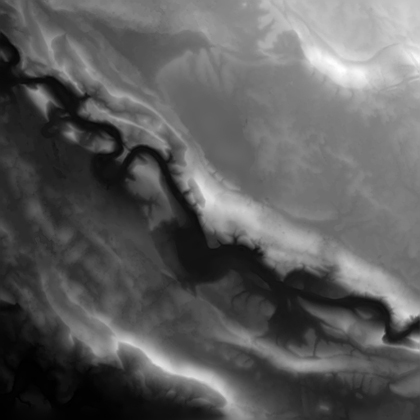
\includegraphics[width=200px]{graphics/heightmap.jpg}
	\caption{In einer Textur abgelegte Höhendaten (Heightmap).}
	\label{fig:heightmap}
\end{figure}

\subsection{Die Darstellung}
Nachdem nun die Grundgeometrie erzeugt, die Höhendaten vor verarbeitet an die GPU übertragen und die Y-Position der Vertices manipuliert wurden, können wir nun unser Terrain endlich darstellen. Einheitlich eingefärbt, bekommen wir allerdings ein Ergebnis dass nicht wirklich an eine Landschaft erinnert (s. Abbildung \ref{fig:singleColors}). 

\begin{figure}[h!]
	\centering
	\vspace*{20px}
	\includegraphics[width=320px]{graphics/singleColor.png}
	\caption{Darstellung mit nur einer Farbe.}
	\label{fig:singleColors}
\end{figure}

Dieses Erscheinungsbild lässt sich durch ein fehlendes Beleuchtungssystem und die dadurch fehlende Schattierung der Szene erklären. Da die Implementierung eines kompletten Beleuchtungssystems für unsere Anwendung allerdings wenig Sinn machen würde, lösen wir das oben gezeigte Darstellungsproblem mit Hilfe von verschiedenen Farben für die unterschiedlichen Höhenwerte. Die einfachste Umsetzung dafür wäre direkt die Farbwerte aus der Höhentextur zu nutzen, wodurch ein Graustufenverlauf von dunkel (niedrig) zu hell (hoch) entstehen würde (s. Abbildung \ref{fig:differentColors}a). Hierdurch erhalten wir zwar eine korrekte Darstellung unseres Terrains, jedoch sind Graustufen mehr als ungeeignet für die spätere Projektion auf den Sand. Aus diesem Grund haben wir eine Möglichkeit zur benutzerdefinierten Wahl des Farbverlaufs implementiert. Diese besteht aus vier frei wählbaren Farben für vier unterschiedliche Höhenbereiche welche im Shader linear interpoliert werden (s. Abbildung \ref{fig:differentColors}b,c).    

\begin{figure}[h!]
	\centering
	\vspace*{30px}
	\includegraphics[width=\textwidth]{graphics/differentColors.png}
	\caption{(a) Einfärbung anhand der Höhentextur. (b, c) Einfärbung anhand eines benutzerdefinierten Farbverlaufs.}
	\label{fig:differentColors}
\end{figure}

Um die Höhenunterschiede bei der Projektion auf den Sand noch deutlicher erkennbar zu machen, haben wir am Ende des ersten Projektsemesters noch mit der Darstellung von Höhenlinien experimentiert und im laufe des zweiten Projektsemester letztendlich vollständig integriert.

Die erste experimentelle Version (s. Abbildung \ref{fig:contourLines}a) arbeitete ausschließlich auf den reinen Höhendaten an einem einzelnen Punkt, weshalb an manchen Stellen noch sehr großflächige, schwarze Bereiche auftraten. Bei der endgültigen Version (s. Abbildung \ref{fig:contourLines}b) flossen schließlich noch zusätzliche Informationen aus den Nachbarbereichen mit in die Berechnung ein, um eine einheitliche Stärke der Höhenlinien zu gewährleisten und größere, schwarze Bereiche auszuschließen.  


\begin{figure}[h!]
	\centering
	\vspace*{50px}
	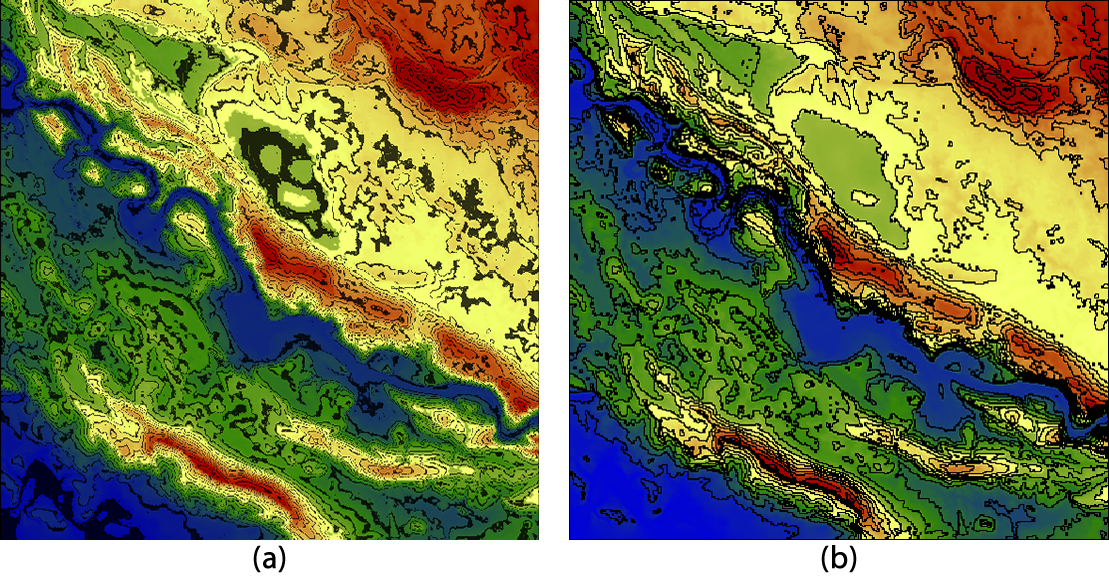
\includegraphics[width=400px]{graphics/contourLines2.png}
	\caption{(a) 1. experimentelle und (b) endgültige Darstellung der Höhenlinien.}
	\label{fig:contourLines}
\end{figure}


\end{Spacing}
\newpage
\clearpage
%% End Of Doc